\documentclass[journal]{IEEEtran}

\usepackage{amsmath,amssymb,amsfonts}
\usepackage{booktabs}
\usepackage{graphicx}
\usepackage{cite}
\usepackage{url}
\usepackage{microtype}
\usepackage{seqsplit}

\begin{document}
\nocite{cliff1993dominance,wilson1927probable,schulman2017proximal}

\title{Supplementary Material: WHOT-ML: A Configurable Partially Observable Multi-Agent Environment for Machine Learning Research}

\author{Brayan~Osinaka%
\thanks{B. Osinaka is an independent researcher based in Benin City, Edo State, Nigeria (e-mail: brayanjunior101@gmail.com).}}

\maketitle

\begin{abstract}
This document provides supplementary empirical datasets, extended ablation tables, full player-count scaling breakdowns, and environment verification telemetry accompanying the main manuscript ``WHOT-ML: A Configurable Partially Observable Multi-Agent Environment for Machine Learning Research.'' All experiments reported herein were executed using containerized cloud infrastructure on the frozen, deterministic reference simulator \texttt{WHOT-NG-v1.0.1}.
\end{abstract}

\section{Player-Count Scaling Dynamics and Telemetry}
\label{sec:supp_player_scaling}

In a standard 54-card WHOT deck with 6-card opening hands and one card dealt face-up to initialize the discard pile, the initial market size is given by $|M_0| = 54 - 1 - (N \times 6) = 53 - 6N$. The cards distributed among the remaining $(N - 1)$ opponents total $|C_{\text{opp}}| = (N - 1) \times 6 = 6N - 6$. We formally define the initial card depletion ratio $\rho_0$ as:
\begin{equation}
\rho_0 = \frac{|C_{\text{opp}}|}{|M_0|} = \frac{6N - 6}{53 - 6N}.
\end{equation}

As summarized in Tables~\ref{tab:supp_exp04a_scaling} and~\ref{tab:supp_exp04b_scaling}, $\rho_0$ increases monotonically from $0.146$ at $N=2$ to $1.765$ at $N=6$, crossing unity between $N=4$ ($\rho_0 = 0.621$) and $N=5$ ($\rho_0 = 1.044$). This marks a critical physical regime shift: for $N \ge 5$, opponents collectively hold more cards than exist in the entire draw market at game inception.

\begin{table*}[t]
\centering
\caption{Player Count Scaling Dynamics: RandomLegal Population (EXP-04a, $N = 2{,}500$ Episodes, 500 Seeds per $N$)}
\label{tab:supp_exp04a_scaling}
\small
\resizebox{\textwidth}{!}{
\begin{tabular}{ccccccccc}
\toprule
$N$ & \textbf{Initial Market} $|M_0|$ & \textbf{Opponent Cards} $|C_{\text{opp}}|$ & \textbf{Ratio} $\rho_0$ & \textbf{Mean Turns} & \textbf{Turns/Player} & \textbf{Mean Draws} & \textbf{Reshuffles} & \textbf{Truncation \% [95\% CI]} \\
\midrule
2 & 41 & 6 & 0.146 & 273.8 & 136.9 & 164.4 & 3.49 & 3.2\% [2.0\%, 5.1\%] \\
3 & 35 & 12 & 0.343 & 296.2 & 98.7 & 186.5 & 4.71 & 2.4\% [1.4\%, 4.2\%] \\
4 & 29 & 18 & 0.621 & 358.3 & 89.6 & 238.7 & 7.85 & 7.0\% [5.1\%, 9.6\%] \\
5 & 23 & 24 & 1.044 & 424.1 & 84.8 & 294.2 & 15.63 & 12.6\% [10.0\%, 15.8\%] \\
6 & 17 & 30 & 1.765 & 451.8 & 75.3 & 320.4 & 31.33 & 12.6\% [10.0\%, 15.8\%] \\
\bottomrule
\end{tabular}
}
\end{table*}

\begin{table*}[t]
\centering
\caption{Player Count Scaling Dynamics: RuleBased Population (EXP-04b, $N = 2{,}500$ Episodes, 500 Seeds per $N$)}
\label{tab:supp_exp04b_scaling}
\small
\resizebox{\textwidth}{!}{
\begin{tabular}{ccccccccc}
\toprule
$N$ & \textbf{Initial Market} $|M_0|$ & \textbf{Opponent Cards} $|C_{\text{opp}}|$ & \textbf{Ratio} $\rho_0$ & \textbf{Mean Turns} & \textbf{Turns/Player} & \textbf{Mean Draws} & \textbf{Reshuffles} & \textbf{Truncation \% [95\% CI]} \\
\midrule
2 & 41 & 6 & 0.146 & 63.9 & 31.9 & 35.2 & 0.41 & 0.0\% [0.0\%, 0.8\%] \\
3 & 35 & 12 & 0.343 & 102.3 & 34.1 & 65.2 & 1.97 & 0.4\% [0.1\%, 1.5\%] \\
4 & 29 & 18 & 0.621 & 489.6 & 122.4 & 438.0 & 244.37 & 41.4\% [37.2\%, 45.8\%] \\
5 & 23 & 24 & 1.044 & 702.9 & 140.6 & 572.5 & 163.04 & 54.6\% [50.2\%, 58.9\%] \\
6 & 17 & 30 & 1.765 & 793.3 & 132.2 & 760.4 & 631.53 & 74.6\% [70.6\%, 78.2\%] \\
\bottomrule
\end{tabular}
}
\end{table*}

\begin{figure}[t]
\centering
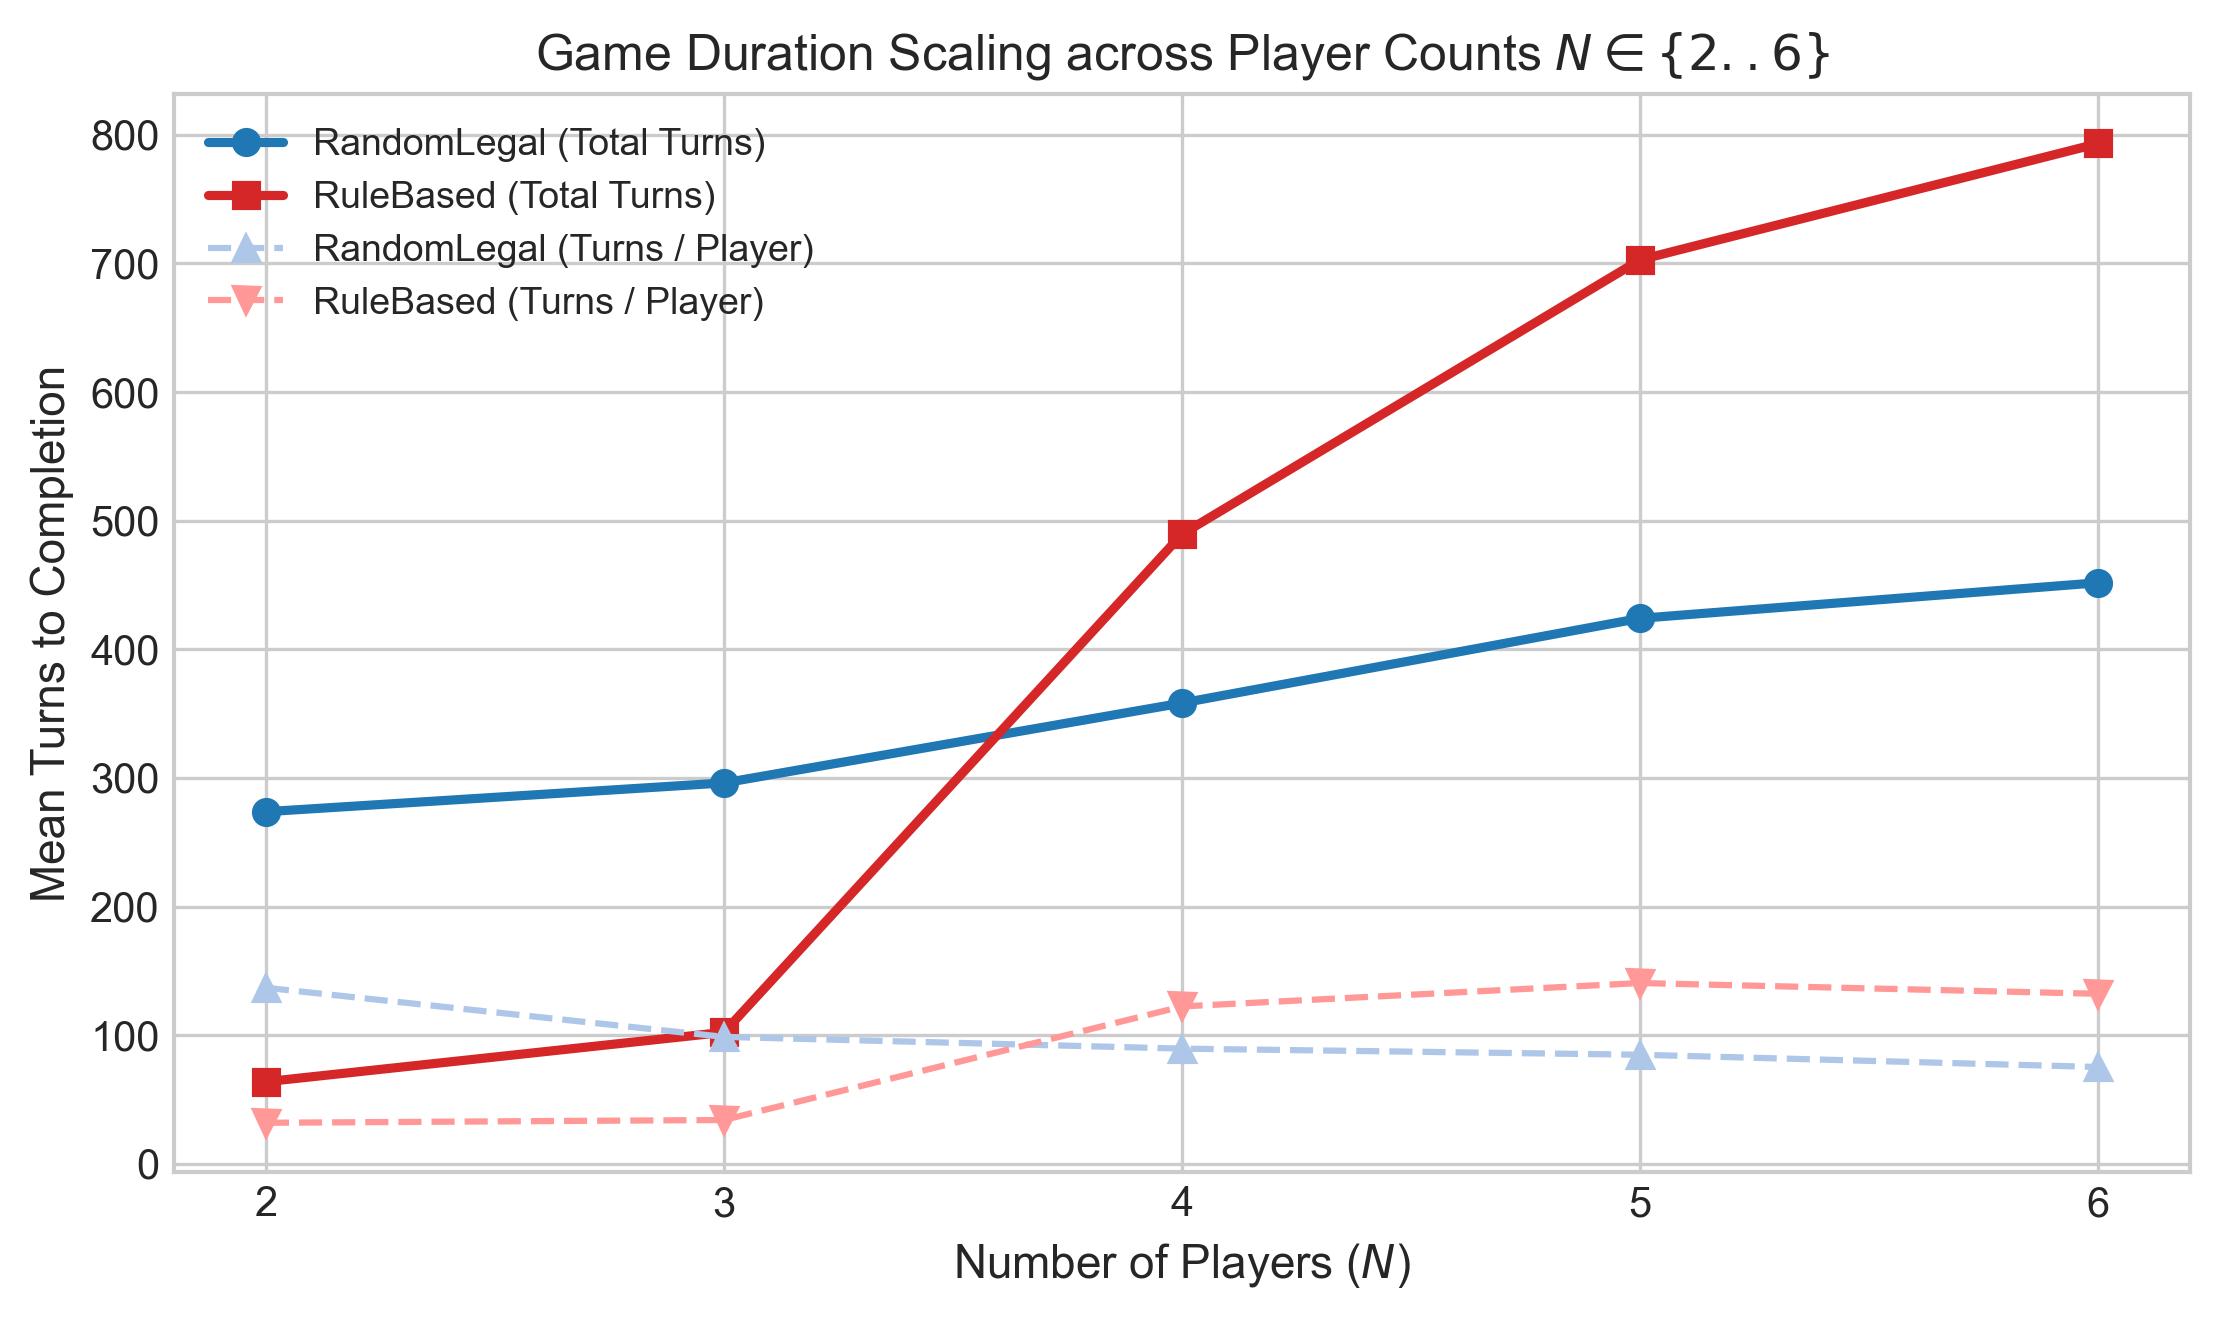
\includegraphics[width=\columnwidth]{figures/fig4_player_scaling_full.png}
\caption{Player Count Scaling Dynamics across $N \in \{2..6\}$ (EXP-04). Side-by-side comparison showing graceful scaling under stochastic legal play (\texttt{RandomLegalAgent}, Table~\ref{tab:supp_exp04a_scaling}) versus catastrophic defensive stall and market collapse under greedy heuristic play (\texttt{RuleBasedAgent}, Table~\ref{tab:supp_exp04b_scaling}).}
\label{fig:supp_fig4_player_scaling}
\end{figure}

Under stochastic legal play (EXP-04a), the environment exhibits graceful linear degradation as player count scales. Mean duration rises moderately from 273.8 turns ($N=2$) to 451.8 turns ($N=6$), while draw counts increase from 164.4 to 320.4. Truncations remain constrained across all regimes, increasing from 3.2\% to 12.6\%. Because random agents do not systematically coordinate or hoard counter-defenses, retaliatory penalty cascades fail to crystallize, permitting games to resolve through natural card shedding.

Conversely, under greedy heuristic self-play (EXP-04b), scaling produces an abrupt phase-like collapse. In two-player ($N=2$) and three-player ($N=3$) regimes, games terminate swiftly (mean 63.9 and 102.3 turns) with virtually no truncations ($\le 0.4\%$). However, at $N=4$, the truncation rate surges to 41.4\% [37.2\%, 45.8\%], escalating further to 54.6\% at $N=5$ and 74.6\% at $N=6$. At $N=6$, games average 631.53 market reshuffles and 760.4 card draws per match. This occurs because as player count expands, the probability that at least one opponent holds an eligible defense card increases sharply, ensuring that any initiated penalty card triggers multi-turn retaliation loops that repeatedly drain and recycle the market deck.

\section{Controlled Rule-Variant Ablation Telemetry}
\label{sec:supp_rule_variants}

To quantify the sensitivity of multi-agent dynamics to rule configurations, EXP-05 evaluated 2,500 games ($N=500$ seeds matched across all variants, seeds 50000--50499) under the verified \texttt{v1.0.1} rules engine in an asymmetric 4-player BRRR setup (1 RuleBased vs. 3 RandomLegal). The evaluated rule variants comprise:
\begin{enumerate}
\item \textbf{\texttt{VAR-BASE}:} Canonical baseline rules with standard Nigerian penalty stacking (\texttt{SAME\_EFFECT}) and mandatory last-card declarations.
\item \textbf{\texttt{VAR-NO-STACK-2}:} Pick-Two penalty stacking disabled (\texttt{NO\_STACKING}); attacked players must draw immediately.
\item \textbf{\texttt{VAR-NO-STACK-3}:} Pick-Three penalty stacking disabled (\texttt{NO\_STACKING}); attacked players must draw immediately.
\item \textbf{\texttt{VAR-NO-DECL}:} Last-card declaration requirement disabled; players may shed their final card without prior announcement.
\item \textbf{\texttt{VAR-PENALTY-2}:} Undeclared last-card victory violation penalty escalated from Draw 1 to Draw 2.
\end{enumerate}

\begin{table*}[t]
\centering
\caption{Controlled Rule Variant Ablations on Simulator v1.0.1 (EXP-05, $N = 2{,}500$ Episodes, 500 Seeds per Variant)}
\label{tab:supp_exp05_rule_variants}
\small
\resizebox{\textwidth}{!}{
\begin{tabular}{llccccc}
\toprule
\textbf{Variant ID} & \textbf{Rule Configuration} & \textbf{Mean Turns} & $\Delta$ \textbf{Turns} & \textbf{Cliff's} $\delta$ & \textbf{RuleBased Win \%} & \textbf{Truncation \% [95\% CI]} \\
\midrule
VAR-BASE & Baseline WHOT-NG-v1 default rules & 223.3 & --- & --- & 66.2\% & 2.2\% [1.2\%, 3.9\%] \\
VAR-NO-STACK-2 & Pick-2 penalty stacking disabled & 226.3 & +3.0 & +0.03 & 63.6\% & 1.4\% [0.7\%, 2.9\%] \\
VAR-NO-STACK-3 & Pick-3 penalty stacking disabled & 227.7 & +4.4 & +0.04 & 65.0\% & 0.8\% [0.3\%, 2.0\%] \\
VAR-NO-DECL & Last-card declaration rule disabled & 173.4 & -49.9 & -0.13 & 53.4\% & 0.8\% [0.3\%, 2.0\%] \\
VAR-PENALTY-2 & Declaration penalty increased Draw 2 & 221.7 & -1.6 & +0.00 & 69.6\% & 1.8\% [1.0\%, 3.4\%] \\
\bottomrule
\multicolumn{7}{l}{\footnotesize \textit{Mean Draws per Episode:} VAR-BASE (151.2), VAR-NO-STACK-2 (150.3), VAR-NO-STACK-3 (149.4), VAR-NO-DECL (118.8), VAR-PENALTY-2 (150.4)} \\
\end{tabular}
}
\end{table*}

\begin{figure}[t]
\centering
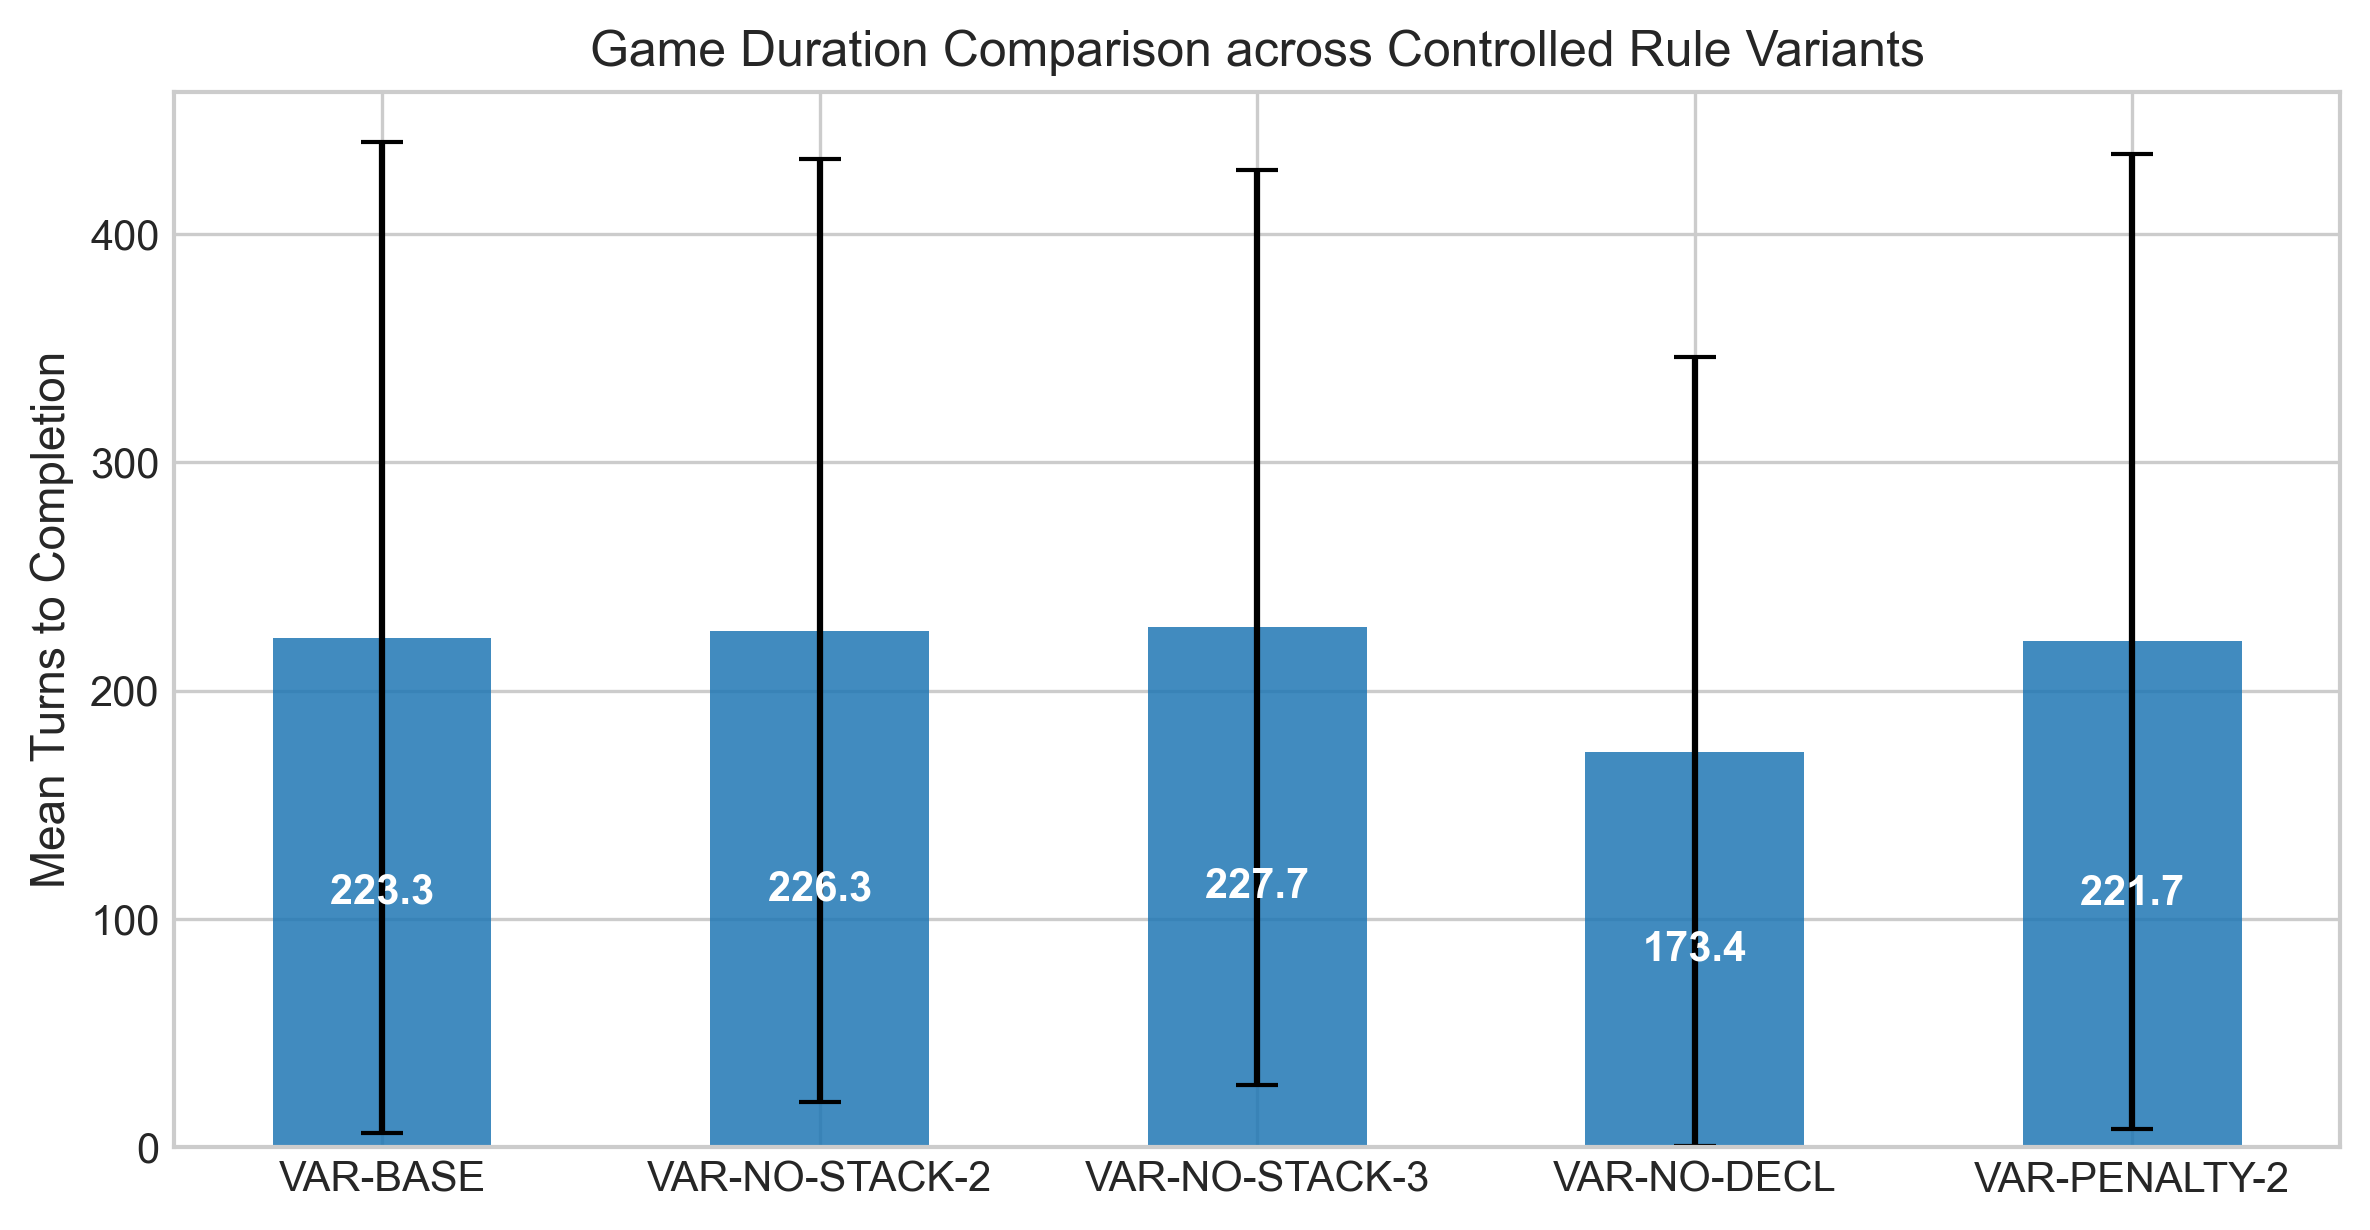
\includegraphics[width=\columnwidth]{figures/fig5_rule_variants_full.png}
\caption{Rule Variant Game Duration Distributions (EXP-05). Paired game duration distributions across five rule variants over 2,500 games (500 seeds each) on simulator v1.0.1, showing the shortening effect of removing declaration requirements and the stabilization of game duration when stacking is prohibited.}
\label{fig:supp_fig5_rule_variants}
\end{figure}

As documented in Table~\ref{tab:supp_exp05_rule_variants} and Figure~\ref{fig:supp_fig5_rule_variants}, eliminating penalty stacking strictly obligates the targeted player to absorb the penalty immediately, eliminating retaliatory counter-chains. Disabling Pick-Three stacking (\texttt{VAR-NO-STACK-3}) cuts the truncation rate from 2.2\% down to 0.8\% [0.3\%, 2.0\%]. Conversely, removing the last-card declaration rule (\texttt{VAR-NO-DECL}) significantly compresses game duration by 49.9 turns ($223.3 \to 173.4$ turns, Cliff's $\delta = -0.13$) and lowers the heuristic win rate from 66.2\% to 53.4\%, demonstrating that declaration mechanics introduce vital strategic friction that informed policies leverage to contain opponents.

\section{Master Results Synthesis}
\label{sec:supp_master_synthesis}

Table~\ref{tab:supp_master_results_synthesis} summarizes the complete experimental campaign across all six empirical investigations, encompassing 16,850 total games, 10,000,000 environment steps of deep reinforcement learning training, and 10,000 diagnostic latent belief probes.

\begin{table*}[t]
\centering
\caption{Master Results Synthesis across EXP-01 through EXP-06 ($N = 16{,}850$ Total Runs + $10{,}000$ Latent Probes)}
\label{tab:supp_master_results_synthesis}
\small
\resizebox{\textwidth}{!}{
\begin{tabular}{lclllc}
\toprule
\textbf{Investigation} & \textbf{Workload} & \textbf{Primary Scientific Finding} & \textbf{Key Empirical Value} & \textbf{Statistical Support} & \textbf{Claim Status} \\
\midrule
EXP-01 & 2,000 & Heuristic expands legal branching factor; & Legal actions: 7.63 vs 2.42; & Mean $\pm$ SD, Median [IQR], & Established \\
(Characterization) & & self-play exhibits emergent defensive stall. & Truncation: 43.6\% vs 7.6\% & Wilson 95\% CIs & \\
\addlinespace
EXP-02 & 449 & Latent state differences produce decisive & Divergence: 84.63\% (380/449); & Wilson 95\% CI [81.0\%, 87.7\%], & Established \\
(Partial Obs.) & & rollout divergence under zero leakage. & Information leakage: 0.0\% & Fisher exact test $p < 10^{-15}$ & \\
\addlinespace
EXP-03 & 5,000 & Heuristic agents dominate random play; & BRRR Win: 65.4\%; BR\_2P Win: 86.3\%; & Unpooled game-level CIs, & Established \\
(Tournaments) & & random agents win 13.7\% in heads-up. & Seating bias: $p = 0.90, p = 0.66$ & Pearson $\chi^2$ test fairness & \\
\addlinespace
EXP-04 & 5,000 & Dynamics undergo regime shift when & Reshuffles: 0.41 $\to$ 631.53; & Paired matched seeds, & Established \\
(Scaling) & & opponent cards exceed market ($\rho_0 > 1$). & Truncation: 0.0\% $\to$ 74.6\% & Monotonic scaling audit & \\
\addlinespace
EXP-05 & 2,500 & Declarations add strategic friction; penalty & NoDecl: $\Delta = -49.9$ turns; & Paired matched seeds, & Established \\
(Ablations) & & stacking drives defensive stalls and recycling. & NoStack: Truncation $2.2\% \to 0.8\%$ & Cliff's $\delta = -0.13, +0.04$ & \\
\addlinespace
Audit & 200 & Simulator certifies determinism, strict & Replays: 100/100; Checkpoints: 100/100; & 114 unit tests passed, & Certified \\
(Determinism) & & privacy boundaries, and state restoration. & RSR = 100.0\% & Bitwise SHA-256 parity & \\
\addlinespace
EXP-06 & 2,000 + 10k & Masked PPO resolves heuristic stall; & PPO Win: 21.2\%; Self-Play Truncation: & Wilson 95\% CIs, & Established \\
(RL \& Probing) & & latent probe reconstructs hidden hands. & 0.5\% (vs 43.6\%); Probe Macro AUROC: 0.5969 (Conditional: 0.5324) & Mann-Whitney AUROC & \\
\bottomrule
\end{tabular}
}
\end{table*}

\section{Environment Determinism and Verification Telemetry}
\label{sec:supp_determinism}

The reference simulator \texttt{WHOT-NG-v1.0.1} was validated against a comprehensive test suite of 114 unit and regression tests. These tests programmatically certify:
\begin{enumerate}
\item \textbf{Card Conservation Invariant:} The total card multiset $\mathbf{H}_t \cup M_t \cup D_t$ equals the canonical 54-card deck $\mathcal{C}_{54}$ at every timestep $t$.
\item \textbf{Information Isolation Invariant:} Observation vectors $O_t^i$ contain strictly zero tokens or indices corresponding to opponent cards $\{H_t^j\}_{j \ne i}$ or market cards $M_t$.
\item \textbf{Bitwise Determinism:} Across 100 complete independent game replays executed under identical seeds, the final game state strings yielded bitwise identical SHA-256 hashes ($100.0\%$ Reproduction Success Rate).
\item \textbf{State Restoration Fidelity:} Across 100 mid-game checkpoints serialized to JSON and subsequently restored into fresh simulator instances, subsequent 20-step rollouts produced bitwise identical event traces and state digests.
\end{enumerate}

The software artifact, full dataset telemetry, and training checkpoints are publicly archived on Zenodo under DOI \url{https://doi.org/10.5281/zenodo.23918026} and GitHub at \url{https://github.com/Brayan114/Project-WHOT}.

\bibliographystyle{IEEEtran}
\bibliography{references}

\end{document}
